% !TeX program = lualatex
% !TeX encoding = utf8
% !BIB program = biber
% !TeX spellcheck = uk_UA

\documentclass{mathreport}
% ------------------------------------------------------------------------------------------------------------
% Add Additional Packages
% ------------------------------------------------------------------------------------------------------------

\renewcommand{\theequation}{\arabic{subsection}.\arabic{equation}}
\renewcommand{\thesubsection}{\arabic{subsection}}

\usepackage{bbm} % for using indicator \mathbbm{1}

% reset equation numbering after each subsection
\counterwithin*{equation}{subsection}

% set page background color (dark read mode)
% \pagecolor[rgb]{0.118,0.118,0.118}
% \color[rgb]{0.8,0.8,0.8}

\begin{document}

\ReportPreamble{Лабораторна робота №1}
\ReportName{Задача статичного\linebreak деформування твердого тіла}
\ReportSubject{Чисельні методи математичної фізики}

\AuthorInfo{Студент 5 курсу, групи КМ-31мн,}
\AuthorName{Цибульник Антон Владиславович}

\SupervisorInfo{Професор кафедри ПМА,}
\SupervisorName{Ориняк Ігор Володимирович}

% warning: in order to fit the text in the very right side of a page, set the longest label
\TheLongestLabel{Цибульник Антон Владиславович}

\import{Title/}{title}

\tableofcontents

\newpage

\section{Постановка задачі}
% \addcontentsline{toc}{section}{Постановка задачі}

У лабораторній роботі розглядається задача деформування тіла певної протяжності --- балки. Опис постановки задачі відповідає так званим крайовим задачам, які розв'язуються одразу для усього одномірного тіла в цілому (на відміну від задач на початкові умови, де пошук розв'язку відбувається крок за кроком, починаючи з певної початкової точки).

Для балки, що згинається, кожна точка $s$ балки довжиною $2L$ характеризується чотирма параметрами: переміщенням $W(s)$, кутом згинання $\theta(s)$, згинальним моментом $M(s)$ та внутрішньою поперечною силою $Q(s)$. Відтак, деформуванню балки відповідатиме така система диференціальних рівнянь:
\begin{align}\label{eq: initial d.e.}
    \frac{dW(s)}{ds} = \theta(s), &&  \frac{d\theta(s)}{ds} = M(s), && \frac{dM(s)}{ds} = Q(s), && \frac{dQ(s)}{ds} = \alpha(s),
\end{align}
де $\alpha(s)$ є зовнішнім навантаження системи. В межах задачі зовнішнє навантаження задається зосередженою силою --- дельта-функцією Дірака $\delta(s-s_0)$, яка приймає нульове значення усюди, окрім околу точки $s_0$, де її значення сягає нескінченності:
\begin{align}\label{eq: delta Dirac}
    \delta(s-s_0)=
    \begin{cases*}
        0, & $s \neq s_0$ \\
        \infty, & $s=s_0$ \\
    \end{cases*}
\end{align}

Крім того, в загальному випадку дельта-функція Дірака $\delta(s)$ володіє такими властивостями:
\begin{align}
    & \int\limits_{\mathbb{R}}\delta(s)\,ds = 1 \label{eq: delta Dirac feature 1} \\
    & \int\limits_{\mathbb{R}}\delta(s-s_0)f(s)\,ds = f(s_0) \label{eq: delta Dirac feature 2}
\end{align}

Отже, моделювання зовнішнього навантаження як зосередженої сили в точці $L/2$ матиме вигляд:
\begin{equation}\label{eq: concentrated force}
    \alpha(s) = \delta(s-L/2),
\end{equation}
а граничні умови задаватимуться рівняннями
\begin{align}\label{eq: edge conditions}
    W(0)=0, && W(2L)=0, && \frac{d^2W(0)}{ds^2}=0, && \frac{d^2W(2L)}{ds^2}=0
\end{align}

Наостанок, балка, яка підлягає деформуванню, згідно з умовами задачі має особливість~--- проміжну опору в точці $L$. Тож на додачу до граничних умов~\eqref{eq: edge conditions} отримуємо обмеження виду
\begin{align}\label{eq: central condition}
    W(L)=0
\end{align}

У подальших викладках буде розглянуто пошук точного аналітичного розв'язку системи рівнянь~\eqref{eq: initial d.e.} методом початкових параметрів (МПП), а для отримання наближеного аналітичного рішення~--- метод зважених залишків (МЗЗ).

\section{Метод початкових параметрів}

\subsection*{Ідея та опис методу}
\addcontentsline{toc}{subsection}{Ідея та опис методу}

Метод початкових параметрів розглядає довільну систему як такі сутності: елементи; межі між елементами (кінці, вузли), де відбувається спряження дотичних елементів; границі всієї системи. При цьому для системи вводиться поняття потужності $N$ --- кількості параметрів, які визначають стан системи в кожній його точці $s$. Виокремлення окреслених вище сутностей системи відбувається поетапно разом із такими супутніми процедурами:

\begin{enumerate}
    \item Система дробиться на декілька окремих ділянок (елементів), і кожна така ділянка нумерується відповідним чином. Після цього визначаються вхідні та вихідні краї кожного елемента, а також вузли --- точки одночасного дотику декількох елементів. Іншими словами, відбувається організація обходу по елементах системи;
    \item Нумерація невідомих змінних (параметрів) на кожному із двох країв кожного елемента системи;
    \item Складання так званих рівнянь зв’язку для кожного елемента. Ці рівняння зв’язують параметри в кінцевій точці елемента зі значеннями в точці початку елемента. Рівняння зв'язку випливають з фізичних чи геометричних властивостей кожного елемента та системи в цілому;
    \item Складання рівнянь спряження в кожному вузлі системи;
    \item Складання рівнянь, що відповідають граничним умовам системи.
\end{enumerate}

Для системи потужності $N$, що складається з $K$ елементів, кількість невідомих параметрів системи складає $2KN$, адже для кожного елемента визначено невідомі змінні (параметри) на його початку та в його кінці. Відповідно, кількість складених рівнянь згідно з методом початкових параметрів має бути $2KN$.  

\newpage
\subsection*{Деталізація поставленої задачі}
\addcontentsline{toc}{subsection}{Деталізація поставленої задачі}

У цьому підрозділі буде почергово розглянуто усі етапи МПП в рамках задачі деформації тіла на площині. Перш за все, з огляду на поставлену крайову задачу~\eqref{eq: initial d.e.}, потужність системи складає $N=4$. Організацію обходу по елементах системи виконаємо таким чином: визначимо $K=2$ елементи та, відповідно, один вузол у точці опори $L$~(Рис.~\ref{pic: beam}).

\vspace{1cm}
\begin{figure}[H]\centering
    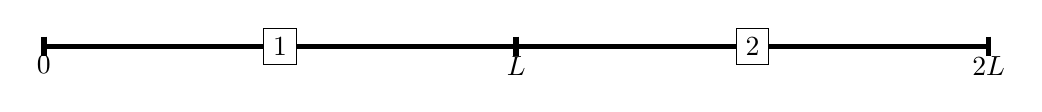
\begin{tikzpicture}
    \pgfmathsetmacro{\L}{6}
    \pgfmathsetmacro{\ticklen}{0.125}

    % element labels
    \node[draw,rectangle] (P1) at (-\L/2,0) {1};
    \node[draw,rectangle] (P2) at (\L/2,0) {2};

    % main line (beam)
    \draw[line width=2pt] (-\L,0) -- (P1) -- (P2) -- (\L,0);

    % ticks
    \draw[line width=2pt] (-\L,\ticklen) -- (-\L,-\ticklen);
    \draw[line width=2pt] (0,\ticklen) -- (0,-\ticklen);
    \draw[line width=2pt] (\L,\ticklen) -- (\L,-\ticklen);

    % labels
    \coordinate[label=below:{$0$}] (E1) at (-\L,0);
    \coordinate[label=below:{$L$}] (E2) at (0,0);
    \coordinate[label=below:{$2L$}] (E3) at (\L,0);
\end{tikzpicture}
    \caption{Балка довжиною $2L$ як система двох елементів}
    \label{pic: beam}
\end{figure}

Дію зовнішнього навантаження~\eqref{eq: concentrated force} на систему~\eqref{eq: initial d.e.} позначено на Рис.~\ref{pic: beam with forces}.

\vspace{1cm}
\begin{figure}[H]\centering
    \begin{tikzpicture}
    \pgfmathsetmacro{\L}{6}
    \pgfmathsetmacro{\ticklen}{0.125}

    % element labels
    % \node[draw,rectangle] (P1) at (-\L/2,0) {1};
    % \node[draw,rectangle] (P2) at (\L/2,0) {2};

    % main line (beam)
    \draw[line width=2pt] (-\L,0) -- (\L,0);

    % ticks
    \draw[line width=2pt] (-\L,\ticklen) -- (-\L,-\ticklen);
    \draw[line width=2pt] (-\L/2,\ticklen) -- (-\L/2,-\ticklen);
    \draw[line width=2pt] (0,\ticklen) -- (0,-\ticklen);
    \draw[line width=2pt] (\L,\ticklen) -- (\L,-\ticklen);

    % labels
    \coordinate[label=below:{$0$}] (E1) at (-\L,0);
    \coordinate[label=above:{$L/2$}] (E2) at (-\L/2,0);
    \coordinate[label=below:{$L$}] (E3) at (0,0);
    \coordinate[label=below:{$2L$}] (E4) at (\L,0);

    % force arrows
    \draw[-{Stealth[scale=1.2]},shorten >= 7.5pt,line width=1.25pt] 
        (-\L/2,-1.4) -- (E2) node[at start,below] {$p_0\,\delta(s-L/2)\cos{\eta t}$};
\end{tikzpicture}
    \caption{Балка під дією зосередженої сили}
    \label{pic: beam with forces}
\end{figure}

Складемо нумерацію невідомих параметрів переміщення $W(s)$, кута згинання $\theta(s)$, згинального моменту $M(s)$ та внутрішньої поперечної сили $Q(s)$ на початку та в кінці кожного елемента (Табл.~\ref{table: element numeration}). В результаті отримаємо $2KN=16$ змінних:

\vspace{0.4cm}
\begin{table}[H]\centering
    \begin{tblr}{
            hlines={1pt,solid}, 
            vlines={1pt,solid},
            hline{4-6}={1-5}{0pt},
            colspec={X[c]X[c]X[c]X[c]X[c]},
            cell{1}{1}={r=2, c=1}{c},
            cell{1}{2}={r=1, c=2}{c},
            cell{1}{4}={r=1, c=2}{c},
            row{3-6}={mode=math},
        }
        
                  & Елемент <<$1$>> & & Елемент <<$2$>> &  \\
                  & Початок & Кінець  & Початок & Кінець   \\
        W(s)      & x_{1}   & x_{5}   & x_{9}   & x_{13}   \\
        \theta(s) & x_{2}   & x_{6}   & x_{10}  & x_{14}   \\
        M(s)      & x_{3}   & x_{7}   & x_{11}  & x_{15}   \\
        Q(s)      & x_{4}   & x_{8}   & x_{12}  & x_{16}   \\

    \end{tblr}
    \caption{Нумерація невідомих параметрів системи}
    \label{table: element numeration}
\end{table}

\newpage
Визначимо рівняння зв'язку, послідовно розглядаючи фізичні рівняння~\eqref{eq: initial d.e.} окремо для кожного елемента. Спершу розглянемо елемент <<$1$>> на проміжку $s \in [0,L]$: враховуючи дію зосередженої сили на другій половині елемента, інтегрування внутрішньої поперечної сили, зважаючи на властивість~\eqref{eq: delta Dirac feature 1} дельта-функції Дірака, буде розписуватися як
\begin{align}\label{eq: Q(s) integrand}
    & Q(s)-Q_0 = \int\limits_{0}^{s} \delta(u-L/2)\, du = \gamma = 
    \begin{cases*}
        0, & $s \in [0,L/2]$ \\ 
        1, & $s \in [L/2,L]$ \\ 
    \end{cases*}
\end{align}

У подальших викладках буде показано, що відповідні рівняння спряження гарантуватимуть неперервність елемента <<$1$>> навіть попри такий розподіл зосередженої сили на різних частинах. Отже, послідовно проінтегруємо й інші фізичні рівняння системи, спираючись на вигляд~\eqref{eq: Q(s) integrand}:
\begin{multline}\label{eq: M(s) integrand}
    M(s)-M_0 = \int\limits_{0}^{s} Q(u)\, du = \int\limits_{0}^{L/2} Q_0\, du + \int\limits_{L/2}^{s} \left( Q_0 + 1 \right) \, du = Q_0 s + \gamma \left( s-\frac{L}{2} \right)
\end{multline}
\begin{multline}\label{eq: theta(s) integrand}
    \theta(s)-\theta_0 = \int\limits_{0}^{s} M(u)\, du = \int\limits_{0}^{L/2} (M_0 + Q_0s)\, du + \int\limits_{L/2}^{s} \left( M_0 + Q_0s + \left( s-\frac{L}{2} \right) \right)\, du = \\
    = M_0 s + Q_0 \frac{s^2}{2} + \gamma \frac{(s-L/2)^2}{2} 
\end{multline}
\begin{multline}\label{eq: W(s) integrand}
    W(s)-W_0 = \int\limits_{0}^{s} \theta(u)\, du = \\
    = \int\limits_{0}^{L/2} \left( M_0 s + Q_0 \frac{s^2}{2} \right)\, du + \int\limits_{L/2}^{s} \left( M_0 s + Q_0 \frac{s^2}{2} + \frac{(s-L/2)^2}{2} \right)\, du = \\
    = \theta_0 s + M_0 \frac{s^2}{2} + Q_0 \frac{s^3}{6} + \gamma \frac{(s-L/2)^3}{6} 
\end{multline}

У матричному вигляді рівняння зв'язку~\eqref{eq: Q(s) integrand} -- \eqref{eq: W(s) integrand} для елемента <<$1$>> записуватимуться таким чином:
\begin{equation}\label{eq: field equations for element 1}
    \begin{pmatrix}
        W(s)      \\
        \theta(s) \\
        M(s)      \\
        Q(s)      \\
    \end{pmatrix} =
    \begin{pmatrix}
        1 & s & \frac{s^2}{2} & \frac{s^3}{6} \\
        0 & 1 & s & \frac{s^2}{2} \\
        0 & 0 & 1 & s \\
        0 & 0 & 0 & 1 \\
    \end{pmatrix}
    \begin{pmatrix}
        W_0      \\
        \theta_0 \\
        M_0      \\
        Q_0      \\
    \end{pmatrix} + \gamma
    \begin{pmatrix}
        \frac{(s-L/2)^3}{6} \\
        \frac{(s-L/2)^2}{2} \\
        s - \frac{L}{2}     \\
        1                   \\
    \end{pmatrix}
\end{equation} 

Тепер розглянемо фізичні рівняння для елемента <<$2$>> на проміжку $s \in [L,2L]$:
\begin{align}
    & Q(s)-Q_L = \int\limits_{L}^{s} 0\, du = 0 \\
    & M(s)-M_L = \int\limits_{L}^{s} Q(u)\, du = \int\limits_{L}^{s} Q_L\, du = Q_L (s-L) \\
    & \theta(s)-\theta_L = \int\limits_{L}^{s} M(u)\, du = M_L (s-L) + Q_L \frac{(s-L)^2}{2} \\
    & W(s)-W_L = \int\limits_{L}^{s} \theta(u)\, du = \theta_L (s-L) + M_L \frac{(s-L)^2}{2} + Q_L \frac{(s-L)^3}{6}
\end{align}

Аналогічним чином матриця рівнянь зв'язку для елемента <<$2$>> матиме вид:
\begin{equation}\label{eq: field equations for element 2}
    \begin{pmatrix}
        W(s)      \\
        \theta(s) \\
        M(s)      \\
        Q(s)      \\
    \end{pmatrix} =
    \begin{pmatrix}
        1 & s-L & \frac{(s-L)^2}{2} & \frac{(s-L)^3}{6} \\
        0 & 1 & s-L & \frac{(s-L)^2}{2} \\
        0 & 0 & 1 & s-L \\
        0 & 0 & 0 & 1 \\
    \end{pmatrix}
    \begin{pmatrix}
        W_L      \\
        \theta_L \\
        M_L      \\
        Q_L      \\
    \end{pmatrix}
\end{equation} 

Підсумовуючи~\eqref{eq: field equations for element 1} та~\eqref{eq: field equations for element 2}, матимемо $8$ рівнянь зв'язку системи в термінах нумерації змінних у Табл.~\ref{table: element numeration}:

\vspace{0.4cm}
\begin{table}[H]\centering
    \begin{tblr}{
            hlines={1pt,solid}, 
            vlines={1pt,solid},
            hline{3-5}={1-2}{0pt},
            colspec={X[l]X[l]},
            rowsep={4pt},
            row{1}={c},
            row{2-5}={l, mode=math, cmd=\quad},
        }
        
        Рівняння зв'язку для елемента <<$1$>> & Рівняння зв'язку для елемента <<$2$>> \\
        x_{5} = x_{1} + x_{2} L + x_{3} \frac{L^2}{2} + x_{4} \frac{L^3}{6} - \frac{L^3}{12} & x_{13} = x_{9} + x_{10}L + x_{11} \frac{L^2}{2} + x_{12} \frac{L^3}{6} \\
        x_{6} = x_{2} + x_{3} L + x_{4} \frac{L^2}{2} & x_{14} = x_{10} + x_{11} L + x_{12} \frac{L^2}{2} \\
        x_{7} = x_{3} + x_{4} L + \frac{L}{2} & x_{15} = x_{11} + x_{12} L \\
        x_{8} = x_{4} + 1 & x_{16} = x_{12} \\

    \end{tblr}
    \caption{Рівняння зв'язку системи}
    \label{table: field equations}
\end{table}

Решта $4$ рівнянь спряження формуватимуться як рівності відповідних змінних внаслідок збереження неперервності у вузлі системи, однак з урахуванням проміжної опори замість рівняння сил виконуватиметься умова нульового переміщення~\eqref{eq: central condition} в точці дотику елементів. Ще $4$ рівняння відповідатимуть граничним умовам~\eqref{eq: edge conditions} системи. Перерахунок рівнянь вказаний у Табл.~\ref{table: transition equations}. 

\begin{table}[H]\centering
    \begin{tblr}{
            hlines={1pt,solid}, 
            vlines={1pt,solid},
            hline{3-5}={1-3}{0pt},
            colspec={X[c]X[c]X[c]},
            row{2-5}={mode=math},
            row{1}={m}
        }
        
        Граничні рівняння зліва & Рівняння спряження & Граничні рівняння справа \\
                                & x_{9}  = x_{5}     &                          \\
        x_{1} = 0               & x_{10} = x_{6}     & x_{13} = 0               \\
        x_{3} = 0               & x_{11} = x_{7}     & x_{15} = 0               \\
                                & x_{9} = 0          &                          \\

    \end{tblr}
    \caption{Рівняння зв'язку та спряження системи}
    \label{table: transition equations}
\end{table} 

\subsection*{Візуалізація отриманих результатів}
\addcontentsline{toc}{subsection}{Візуалізація отриманих результатів}

Розв'язавши систему та отримавши величини невідомих змінних (Табл.~\ref{table: element numeration}), маємо змогу використати рівняння зв'язку~\eqref{eq: field equations for element 1} та~\eqref{eq: field equations for element 2} для отримання аналітичних проміжних значень параметра переміщення при деформації балки довжиною $2L=100$ під дією зосередженої сили в точці $L/2$ і з урахуванням проміжної опори в точці $L$ (Рис.~\ref{pic: TMM}). У Табл.~\ref{table: element values} зазначені отримані значення змінних системи.

\vspace{0.4cm}
\begin{figure}[H]\centering
    \resizebox{\linewidth}{!}{\begin{tikzpicture}
    \begin{axis}[
        height = 0.5\linewidth,
        width = 0.85\linewidth,
        xlabel={Координата балки $s$},
        ylabel={Значення переміщення $W(s)$},
        scale only axis,
        scaled y ticks=false,
        xmin=-5, xmax=105,
        ymin=-1125, ymax=2125, 
        % ytick distance=0.001,
        % yticklabel style={
        %     /pgf/number format/.cd,
        %     fixed,
        %     precision=3
        % }, % set fixed precision of 2 decimal places
        grid=both,
        grid style={draw=gray!30},
        minor grid style={draw=gray!10},
        minor x tick num=3,
        minor y tick num=3,
    ]
        \addplot[gray!50, dash pattern={on 7pt off 4pt}, line width=1pt] table {
            -10 0
            110 0
        };
        \addplot[blue!80, line width=2pt] table {Data/TMM.txt};
        \addplot[blue!80, only marks, mark=*, mark size=3pt] table {
            0 0
            50 0
            100 0
        };

    \end{axis}
\end{tikzpicture}}
    % \includegraphics[width=\linewidth]{Tikzplots/TMM.tikz}
    \caption{Крива деформації за методом МПП}
    \label{pic: TMM}
\end{figure}

\begin{table}[H]\centering
    \begin{tblr}{
            hlines={1pt,solid}, 
            vlines={1pt,solid},
            hline{4-6}={1-5}{0pt},
            colspec={X[c]X[l]X[l]X[l]X[l]},
            cell{1}{1}={r=2, c=1}{c},
            cell{1}{2}={r=1, c=2}{c},
            cell{1}{4}={r=1, c=2}{c},
            row{2}={c},
            row{3-6}={mode=math},
        }
        
                  & Елемент <<$1$>> &                & Елемент <<$2$>>  &               \\
                  & Початок         & Кінець         & Початок          & Кінець        \\
        W(s)      & x_{1}=0         & x_{5}=0        & x_{9}=0          & x_{13}=0      \\
        \theta(s) & x_{2}=117.188   & x_{6}=-78.125  & x_{10}=-78.125   & x_{14}=39.063 \\
        M(s)      & x_{3}=0         & x_{7}=4.688    & x_{11}=4.688     & x_{15}=0      \\
        Q(s)      & x_{4}=-0.406    & x_{8}=0.594    & x_{12}=-0.094    & x_{16}=-0.094 \\

    \end{tblr}
    \caption{Значення змінних системи за методом МПП}
    \label{table: element values}
\end{table}

\section{Метод зважених залишків}

\subsection*{Ідея та опис методу}
\addcontentsline{toc}{subsection}{Ідея та опис методу}

Метод зважених залишків оперує рівнянням вигляду
\begin{equation}\label{eq: G(y) = f(x)}
    G(y) = f(x),
\end{equation}
де $G(y)$~--- деякий заданий лінійний диференціальний оператор над функцією $y(x)$, а $f(x)$ у правій частині є певним зовнішнім навантаженням (дією зовнішніх сил). Припускається, що функція $y(x)$ має форму суми $M$ так званих базових функцій $\phi_i(x)$, помножених на невідомі коефіцієнти $a_i$:
\begin{equation}\label{eq: y(x) approximation}
    y(x) = \sum\limits_{i=1}^{M} a_i\phi_i(x)
\end{equation}

Зауважимо, що перелік базових функцій задається так, щоб задовольнити нульові граничні умови задачі. Отже, оскільки вигляд~\eqref{eq: y(x) approximation}~--- лише наближення невідомої функції $y(x)$, вводиться поняття залишку диференціального оператора:
\begin{equation}\label{eq: R(x) residual}
    R(x) = \sum\limits_{i=1}^{M} a_i G\bigl( \phi_i(x) \bigr) - f(x)
\end{equation}

Мета методу полягає у мінімізації утвореного залишку $R(x)$ шляхом пошуку оптимальних значень коефіцієнтів $a_i$ через почергову процедуру <<зваження>> з кожною базовою функцією $\phi_i(x)$:
\begin{equation}\label{eq: R(x) minimizing}
    \int\limits_{\mathbb{R}} R(x)\, \phi_i(x)\, dx = 0,\ i=\overline{1,M}
\end{equation}

Таким чином, кількість рівнянь~\eqref{eq: R(x) minimizing} дорівнює кількості невідомих коефіцієнтів $a_i$, що дозволяє розв'язати утворену систему рівнянь та отримати наближене аналітичне рішення згідно з припущенням~\eqref{eq: y(x) approximation}.

\subsection*{Деталізація поставленої задачі}
\addcontentsline{toc}{subsection}{Деталізація поставленої задачі}

Для того, щоб застосувати метод зважених залишків до заданої задачі деформування, слід виконати деякі модифікації та уточнення системи~\eqref{eq: initial d.e.}. Перш за все, задля введення сутності диференціального оператора систему необхідно звести до диференціального рівняння четвертого порядку відносно параметра переміщення $W(s)$. 

Наступним кроком є моделювання проміжної точки опори балки як дії зосередженої сили з невідомою інтенсивністю $z$~--- дельта-функції Дірака в точці $L$. Відтак, задача з граничними умовами~\eqref{eq: edge conditions} описуватиметься таким рівнянням:
\begin{equation}\label{eq: united initial d.e.}
    \frac{d^4W(s)}{ds^4} = \delta(s-L/2) + z\delta(s-L),
\end{equation}
тоді у введених раніше термінах
\begin{align}\label{eq: G(W)}
    & G(W) = \frac{d^4W(s)}{ds^4} \\
    & f(s) = \delta(s-L/2) + z\delta(s-L)
\end{align}

Наближений аналітичний вигляд функції переміщення $W(s)$ покладемо так:
\begin{equation}\label{eq: W(s) M=2 approximation}
    W(s) = a_1\phi_1(s) + a_2\phi_2(s),
\end{equation}
де набір з $M=2$ базових функцій обрано з експоненціальної сім'ї:
\begin{align}
    & \phi_1(s) = e^{-\frac{4s}{2L}} + C_{11}e^{-\frac{3s}{2L}} + C_{12}e^{-\frac{2s}{2L}} + C_{13}e^{-\frac{s}{2L}} + C_{14}, \label{eq: M=2 trial phi1(x)} \\
    & \phi_2(s) = e^{-\frac{3s}{2L}} + C_{21}e^{-\frac{2s}{2L}} + C_{22}e^{-\frac{s}{2L}} + C_{23} + C_{24}e^{\frac{s}{2L}} \label{eq:  M=2 trial phi2(x)},
\end{align}
при цьому в силу нульових граничних умов~\eqref{eq: edge conditions} коефіцієнти $C_{ij}$ дорівнюють:

\vspace{0.4cm}
\begin{table}[H]\centering
    \begin{tblr}{
            % hline{2}={1pt,solid},
            % vline{2-8}={1pt,solid},
            hlines={1pt,solid},
            vlines={1pt,solid},
            colspec={X[c]X[c]X[c]X[c]X[c]X[c]X[c]X[c]},
            row{1-2}={mode=math},
        }
        
        C_{11}  & C_{12} & C_{13} & C_{14}  & C_{21}  & C_{22} & C_{23}  & C_{24} \\
        -2.2834 & 1.0149 & 0.4912 & -0.2227 & -2.9305 & 2.6637 & -0.7915 & 0.0583 \\

    \end{tblr}
    \caption{Значення коефіцієнтів базових функцій~\eqref{eq: M=2 trial phi1(x)} й \eqref{eq: M=2 trial phi2(x)}}
    \label{table: A coefficients values}
\end{table}

Враховуючи наведену формалізацію системи, залишок матиме вид:
\begin{equation}\label{eq: R(x) residual for W(s)}
    R(s) = a_1 \frac{d^4\phi_1(s)}{ds^4} + a_2 \frac{d^4\phi_2(s)}{ds^4} - \delta(s-L/2) - z\delta(s-L)
\end{equation}

\newpage
Тоді з урахуванням умови~\eqref{eq: central condition} нульового переміщення в точці опори, система рівнянь~\eqref{eq: R(x) minimizing} для визначення невідомих коефіцієнтів $a_1,a_2$ та $z$ згідно з методом зважених залишків записуватиметься на проміжку від $0$ до $2L$ таким чином:
\begin{align}
    & \int\limits_{0}^{2L} R(s)\, \phi_1(s)\, ds = 0, \\
    & \int\limits_{0}^{2L} R(s)\, \phi_2(s)\, ds = 0, \\
    & W(L) = 0, 
\end{align}
що розписується у систему 
\begin{align}
    & a_1\int\limits_{0}^{2L} \phi_1^{(4)}(s)\, \phi_1(s)\, ds + a_2\int\limits_{0}^{2L} \phi_2^{(4)}(s)\, \phi_1(s)\, ds- z\phi_1(L)-\phi_1(L/2) = 0 \\
    & a_1\int\limits_{0}^{2L} \phi_1^{(4)}(s)\, \phi_2(s)\, ds + a_2\int\limits_{0}^{2L} \phi_2^{(4)}(s)\, \phi_2(s)\, ds- z\phi_2(L)-\phi_2(L/2) = 0 \\
    & a_1\phi_1(L) + a_2\phi_2(L) = 0
\end{align}

Позначивши відповідні визначені інтеграли через позначки $I_{ij}$, отримані рівняння компактно записуються у матричному вигляді:
\begin{equation}\label{eq: residuals matrix equation}
    \begin{pmatrix}
        I_{11}    & I_{21}    & -\phi_1(L) \\
        I_{12}    & I_{22}    & -\phi_2(L) \\
        \phi_1(L) & \phi_2(L) & 0          \\
    \end{pmatrix}
    \begin{pmatrix}
        a_1 \\
        a_2 \\
        z \\
    \end{pmatrix} = 
    \begin{pmatrix}
        \phi_1(L/2) \\
        \phi_2(L/2) \\
        0           \\
    \end{pmatrix}
\end{equation} 

Виконавши відповідні обчислення визначених інтегралів та розв'язавши матричне рівняння~\eqref{eq: residuals matrix equation}, отримуємо такі результати:

\vspace{0.4cm}
\begin{table}[H]\centering
    \begin{tblr}{
        hlines={1pt,solid},
        vlines={1pt,solid},
            colspec={ccc},
            row{1-2}={mode=math},
        }
        
        a_{1}  & a_{2} & z \\
        339543.2272 & -387324.2929 & -0.6980 \\

    \end{tblr}
    \caption{Значення невідомих коефіцієнтів функції~\eqref{eq: W(s) M=2 approximation}}
    \label{table: W(s) coefficients values}
\end{table}

\newpage
\subsection*{Візуалізація отриманих результатів}
\addcontentsline{toc}{subsection}{Візуалізація отриманих результатів}

Використовуючи знайдені значення коефіцієнтів $a_1$ та $a_2$ з Табл.~\ref{table: W(s) coefficients values} й скориставшись формулою наближеного аналітичного розв'язку~\eqref{eq: W(s) M=2 approximation}, маємо змогу побудувати неперервні значення переміщення при деформації балки довжиною $2L=100$ під дією зосередженої сили в точці $L/2$ з урахуванням проміжної опори в точці $L$. 

Порівняльний графік кривих за аналітичним методом МПП та наближеним аналітичним рішенням МЗЗ наведений на Рис~\ref{pic: TMM vs WRM (M=2)}. Міру несхожості отриманих кривих $W(s)_{\text{мпп}}$ та $W(s)_{\text{мзз}}$ визначатимемо так:
\begin{equation}\label{eq: measure of dissimilarity}
    \Delta W(s) = \frac{1}{|I|} \sum\limits_{i \in I} \left| \frac{ W(s_i)_{\text{мпп}} - W(s_i)_{\text{мзз}}}{W(s_i)_{\text{мпп}}} \right|,\ I=\{1,2,\ldots,2L\}
\end{equation}

\begin{figure}[H]\centering
    \resizebox{\linewidth}{!}{\begin{tikzpicture}
    \begin{axis}[
        height = 0.5\linewidth,
        width = 0.85\linewidth,
        xlabel={Координата балки $s$},
        ylabel={Значення переміщення $W(s)$},
        scale only axis,
        scaled y ticks=false,
        xmin=-5, xmax=105,
        ymin=-1125, ymax=2125, 
        % ytick distance=0.001,
        % yticklabel style={
        %     /pgf/number format/.cd,
        %     fixed,
        %     precision=3
        % }, % set fixed precision of 2 decimal places
        yticklabel style={
            /pgf/number format/.cd,
            1000 sep={},
        },
        grid=both,
        grid style={draw=gray!30},
        minor grid style={draw=gray!10},
        minor x tick num=3,
        minor y tick num=3,
        reverse legend,
        legend style={                       % customize the legend style
            at={(0.95,0.95)},                % position the legend at the top right corner of the plot
            font=\small,                     % set the font size of the legend
            anchor=north east,               % anchor the legend to the north east corner
            cells={anchor=west}              % align the legend text to the left
        },
    ]
        \addplot[gray!50, dash pattern={on 7pt off 4pt}, line width=1pt, forget plot] table {
            -10 0
            110 0
        };

        \addplot[orange!80, line width=2pt] table {Data/WRM (M=2).txt};
        \addlegendentry{\ Метод МЗЗ $(M=2)$}
        \addplot[blue!80, line width=2pt] table {Data/TMM.txt};
        \addlegendentry{\ Метод МПП}

        \addplot[blue!80, only marks, mark=*, mark size=3pt, forget plot] table {
            0 0
            50 0
            100 0
        };

    \end{axis}
\end{tikzpicture}}
    % \includegraphics[width=\linewidth]{Tikzplots/TMM.tikz}
    \caption{Порівняльний графік кривих деформації за МПП та МЗЗ при виборі $M=2$ базових функцій вигляду~\eqref{eq: M=2 trial phi1(x)} й \eqref{eq: M=2 trial phi2(x)}}
    \label{pic: TMM vs WRM (M=2)}
\end{figure}

Згідно з~\eqref{eq: measure of dissimilarity}, міра несхожості між кривими на Рис.~\ref{pic: TMM vs WRM (M=2)} складатиме:
\begin{equation}\label{eq: measure of dissimilarity (M=2) value}
    \Delta W(s) = 15.86\%
\end{equation}

\subsection*{Коригування набору базових функцій}
\addcontentsline{toc}{subsection}{Коригування набору базових функцій}

Розглянемо почергово дещо доповнені переліки базових функцій з експоненціальної сім'ї. А саме, почнемо з набору $M=3$ базових функцій виду:
\begin{align}
    & \phi_1(s) = e^{-\frac{4s}{2L}} + C_{11}e^{-\frac{3s}{2L}} + C_{12}e^{-\frac{2s}{2L}} + C_{13}e^{-\frac{s}{2L}} + C_{14}, \label{eq: M=3 trial phi1(x)} \\
    & \phi_2(s) = e^{-\frac{3s}{2L}} + C_{21}e^{-\frac{2s}{2L}} + C_{22}e^{-\frac{s}{2L}} + C_{23} + C_{24}e^{\frac{s}{2L}}, \label{eq: M=3 trial phi2(x)} \\
    & \phi_3(s) = e^{-\frac{2s}{2L}} + C_{31}e^{-\frac{s}{2L}} + C_{32} + C_{33}e^{\frac{s}{2L}} + C_{34}e^{\frac{2s}{2L}}, \label{eq: M=3 trial phi3(x)}
\end{align}
які в силу задовольнення нульових граничних умов~\eqref{eq: edge conditions} матимуть визначені коефіцієнти $C_{ij}$. Аналогічним чином провівши процедуру <<зваження>> за МЗЗ, отримаємо шукані коефіцієнти $a_1,a_2,a_3$ для представлення функції переміщення у вигляді: 
\begin{equation}\label{eq: W(s) M=3 approximation}
    W(s) = a_1\phi_1(s) + a_2\phi_2(s) + a_3\phi_3(s)
\end{equation}

Отримана крива проілюстрована на Рис.~\ref{pic: TMM vs WRM}, значення міри несхожості з результатами МПП зображені у Табл.~\ref{table: measure of dissimilarity}. Наступний набір $M=4$ базових функцій покладемо як 
\begin{align}
    & \phi_1(s) = e^{-\frac{4s}{2L}} + C_{11}e^{-\frac{3s}{2L}} + C_{12}e^{-\frac{2s}{2L}} + C_{13}e^{-\frac{s}{2L}} + C_{14}, \label{eq: M=4 trial phi1(x)} \\
    & \phi_2(s) = e^{-\frac{3s}{2L}} + C_{21}e^{-\frac{2s}{2L}} + C_{22}e^{-\frac{s}{2L}} + C_{23} + C_{24}e^{\frac{s}{2L}}, \label{eq: M=4 trial phi2(x)} \\
    & \phi_3(s) = e^{-\frac{2s}{2L}} + C_{31}e^{-\frac{s}{2L}} + C_{32} + C_{33}e^{\frac{s}{2L}} + C_{34}e^{\frac{2s}{2L}}, \label{eq: M=4 trial phi3(x)} \\
    & \phi_4(s) = e^{-\frac{s}{2L}} + C_{41} + C_{42}e^{\frac{s}{2L}} + C_{43}e^{\frac{2s}{2L}} + C_{44}e^{\frac{3s}{2L}}, \label{eq: M=4 trial phi4(x)}
\end{align}
які, своєю чергою, задовольняють нульовим граничним умовам~\eqref{eq: edge conditions} та формують функцію переміщення відповідно до~\eqref{eq: y(x) approximation}:
\begin{equation}\label{eq: W(s) M=4 approximation}
    W(s) = a_1\phi_1(s) + a_2\phi_2(s) + a_3\phi_3(s) + a_4\phi_4(s)
\end{equation}

Усі порівняльні характеристики кривої продемонстровані на Рис.~\ref{pic: TMM vs WRM} та у Табл.~\ref{table: measure of dissimilarity}. Зауважуємо, що наближений аналітичний розв'язок при $M=4$ вже значно точніше апроксимує криву за методом МПП. Наостанок, розглянемо набір таких $M=5$ базових функцій, які задовольняють усім умовам МЗЗ:
\begin{align}
    & \phi_1(s) = e^{-\frac{4s}{2L}} + C_{11}e^{-\frac{3s}{2L}} + C_{12}e^{-\frac{2s}{2L}} + C_{13}e^{-\frac{s}{2L}} + C_{14} \label{eq: M=5 trial phi1(x)} \\
    & \phi_2(s) = e^{-\frac{3s}{2L}} + C_{21}e^{-\frac{2s}{2L}} + C_{22}e^{-\frac{s}{2L}} + C_{23} + C_{24}e^{\frac{s}{2L}} \label{eq: M=5 trial phi2(x)} \\
    & \phi_3(s) = e^{-\frac{2s}{2L}} + C_{31}e^{-\frac{s}{2L}} + C_{32} + C_{33}e^{\frac{s}{2L}} + C_{34}e^{\frac{2s}{2L}} \label{eq: M=5 trial phi3(x)} \\
    & \phi_4(s) = e^{-\frac{s}{2L}} + C_{41} + C_{42}e^{\frac{s}{2L}} + C_{33}e^{\frac{2s}{2L}} + C_{44}e^{\frac{3s}{2L}} \label{eq: M=5 trial phi4(x)} \\
    & \phi_5(s) = 1 + C_{51}e^{\frac{s}{2L}} + C_{52}e^{\frac{2s}{2L}} + C_{53}e^{\frac{3s}{2L}} + C_{54}e^{\frac{4s}{2L}} \label{eq: M=5 trial phi5(x)}
\end{align}

\begin{figure}[H]\centering
    \resizebox{\linewidth}{!}{\begin{tikzpicture}
    \begin{axis}[
        height = 0.5\linewidth,
        width = 0.85\linewidth,
        xlabel={Координата балки $s$},
        ylabel={Значення переміщення $W(s)$},
        scale only axis,
        scaled y ticks=false,
        xmin=-5, xmax=105,
        ymin=-1125, ymax=2125, 
        % ytick distance=0.001,
        % yticklabel style={
        %     /pgf/number format/.cd,
        %     fixed,
        %     precision=3
        % }, % set fixed precision of 2 decimal places
        grid=both,
        grid style={draw=gray!30},
        minor grid style={draw=gray!10},
        minor x tick num=3,
        minor y tick num=3,
        reverse legend,
        legend style={                       % customize the legend style
            at={(0.95,0.95)},                % position the legend at the top right corner of the plot
            font=\small,                     % set the font size of the legend
            anchor=north east,               % anchor the legend to the north east corner
            cells={anchor=west}              % align the legend text to the left
        },
    ]
        \addplot[gray!50, dash pattern={on 7pt off 4pt}, line width=1pt, forget plot] table {
            -10 0
            110 0
        };

        \addplot[black!80, line width=2pt] table {Data/WRM (M=5).txt};
        \addlegendentry{\ Метод МЗЗ $(M=5)$}
        \addplot[purple!80, line width=2pt] table {Data/WRM (M=4).txt};
        \addlegendentry{\ Метод МЗЗ $(M=4)$}
        \addplot[green!60!black, line width=2pt] table {Data/WRM (M=3).txt};
        \addlegendentry{\ Метод МЗЗ $(M=3)$}
        \addplot[orange!80, line width=2pt] table {Data/WRM (M=2).txt};
        \addlegendentry{\ Метод МЗЗ $(M=2)$}
        \addplot[blue!80, line width=2pt] table {Data/TMM.txt};
        \addlegendentry{\ Метод МПП}

        \addplot[blue!80, only marks, mark=*, mark size=3pt, forget plot] table {
            0 0
            50 0
            100 0
        };

    \end{axis}
\end{tikzpicture}}
    % \includegraphics[width=\linewidth]{Tikzplots/TMM.tikz}
    \caption{Порівняльний графік кривих деформації за МПП та МЗЗ при виборі різної кількості $M$ базових функцій експоненціальної сім'ї}
    \label{pic: TMM vs WRM}
\end{figure}

Результати при $M=5$ (Табл.~\ref{table: measure of dissimilarity}) мають найменше відхилення від кривої, отриманої за методом МПП~--- лише $3.12\%$. 

\vspace{0.4cm}
\begin{table}[H]\centering
    \begin{tblr}{
            hlines={1pt,solid},
            vlines={1pt,solid},
            colspec={cQ[2cm,c]Q[2cm,c]Q[2cm,c]Q[2cm,c]},
            rows={mode=math},
        }
        
                    & M=2     & M=3     & M=4     & M=5    \\ 
        \Delta W(s) & 15.86\% & 19.26\% & 10.22\% & 3.12\% \\

    \end{tblr}
    \caption{Значення міри несхожості між кривими за МПП та МЗЗ при виборі різної кількості $M$ базових функцій експоненціальної сім'ї}
    \label{table: measure of dissimilarity}
\end{table}

\newpage
\section{Висновки}

У лабораторній роботі було розглянуто крайову задачу деформування тіла протяжності $2L$~--- балки. Балка за умовами задачі має проміжну опору в точці $L$ та дію зосередженої сили в точці $L/2$. Кожна точка $s$ балки характеризується чотирма параметрами: переміщенням $W(s)$, кутом згинання $\theta(s)$, згинальним моментом $M(s)$ та внутрішньою поперечною силою $Q(s)$.

Для пошуку аналітичного розв'язку системи диференціальних рівнянь, які описують деформацію балки, було використано метод початкових параметрів: тіло структурно було розділено на два елементи та один вузол. На кожному елементі були складені рівняння зв'язку для невідомих параметрів системи із урахуванням дії зосередженої сили в точці $L/2$. Враховуючи проміжну опору, також були складені рівняння спряження у вузлі системи та рівняння, які відповідають граничним умовам. Розв'язавши систему складених рівнянь, вдалося отримати неперервний розв'язок для задачі деформування балки, який відповідає логіці процесу згинання під дією зосередженої сили з проміжною опорою.  

Для пошуку наближеного аналітичного розв'язку було використано метод зважених залишків. Було отримано декілька різних наближених кривих, які почергово включали різну кількість базових функцій з експоненціальної сім'ї. Найкраще наближення вдалося отримати при розгляді п'ятьох базових функцій~--- лише $3.12\%$ відхилення.

\newpage
\section{Програмна реалізація}

В ході дослідження було використано засоби мови програмування \texttt{Python} версії \texttt{3.8.10} в інтегрованому середовищі розробки \texttt{Visual Studio Code} версії \texttt{1.78.2}. Нижче наведені тексти ключових інструментальних програм.

\lstinputlisting[linerange={1-5}, caption={Підключення бібліотек та ініціалізація параметрів}]{Code/code.py}

\lstinputlisting[linerange={11-57}, caption={Реалізація методу початкових параметрів (МПП)}]{Code/code.py}

\lstinputlisting[linerange={63-85}, caption={Визначення коефіцієнтів базових функцій (МЗЗ)}]{Code/code.py}

\lstinputlisting[linerange={87-98}, caption={Введення допоміжних функцій (МЗЗ)}]{Code/code.py}

\lstinputlisting[linerange={100-126}, caption={Обчислення невідомих коефіцієнтів системи (МЗЗ)}]{Code/code.py}

\lstinputlisting[linerange={128-133}, caption={Візуалізація отриманих результатів (МЗЗ)}]{Code/code.py}

% \newpage
% \printbibliography[title={Перелік посилань}] % \nocite{*}
% \addcontentsline{toc}{subsection}{Перелік посилань}

\end{document}